\chapter{Estimación del número de señales recibidas}\label{ch:machinelearning}
\chapterquote{Comin' at you from every side...}{Mike Shinoda}

\section{Introducción}\label{subc:intro_congen}
Una gran capacidad que tienen los sistemas de conformación de haz digitales frente a los analógicos es la de poder realizar la conformación de más de una señal simultáneamente utilizando un único sistema. Además, la versión adaptativa de este tipo de conformadores de haz permiten no solo ajustarse automáticamente a cambios en las direcciones de arribo de las señales sino, además, poder estimar qué cantidad de señales están siendo sensadas por los elementos del arreglo de antenas. Esta magnitud es de extrema importancia en todos los algoritmos de estimación de dirección de arribo ya que define todas las dimensiones de las matrices con las que se debe operar, comenzando por las matrices $\mathbf{\hat{E}_S}$ y $\mathbf{\hat{E}_W}$ definidas en la Ecuación \ref{eq:doaest_es_en}, que son las matrices conformadas por las estimaciones de los autovectores de los subespacios de señal y ruido respectivamente.

Como se indicó en la Sección \ref{subc:doaest_datamodel} el problema de estimar la cantidad de señales recibidas consiste en separar los valores singulares obtenidos mediante la SVD de la matriz $\mathbf{X}$ definida en la Ecuación \ref{eq:doaest_x} entre aquellos de mayor valor, los cuales corresponden a los valores singulares del subespacio de señal, y aquellos más chicos, que corresponden al subespacio de ruido. En el caso ideal en el que ambos subespacios pueden ser estimados perfectamente esta tarea no conlleva mayor dificultad debido a que los valores singulares del subespacio de ruido tienen todos la misma magnitud, por ende es fácil separarlos del resto. En la práctica, cuando lo que se tiene son estimaciones de estos subespacios, esta característica no se observa y las magnitudes de los valores singulares del subespacio de ruido pueden diferir entre ellos.

En la Figura \ref{fig:ml_aval} se muestra una simulación en la que se obtuvieron los valores singulares de una matriz de muestras $\mathbf{X}$ armada a partir de la recepción hecha por un ARU de $M=16$ elementos de dos señales en direcciones distintas con una SNR de 10 dB cada una.
\begin{figure}[ht!]
  \centering
  \includegraphics[width=0.9\linewidth]{images/05-Machine Learning/ml_aval.png}
  \caption{Distribución de valores singulares del subespacio de muestras ordenados de mayor a menor para el caso de dos señales arribando a un arreglo de 16 elementos. La línea azul indica la separación entre valores singulares correspondientes al subespacio de señal y al subespacio de ruido.}
  \label{fig:ml_aval}
\end{figure}
Como puede verse, en este caso se puede determinar fácilmente un umbral a partir del cual cualquier valor singular que esté por encima sea considerado como correspondiente al subespacio de señal. Sin embargo, la práctica demuestra que este umbral no es constante sino que varía según las características de la señal recibida, como lo son la SNR de las mismas, la cantidad de señales a detectar y cuán correlacionadas se encuentran entre ellas, por ende esta propuesta no es aplicable en general.

En este capítulo se presentan y comparan dos métodos de estimación de número de señales recibidas que se basan en el análisis de los valores singulares del subespacio de muestras.


\section{Método de la máxima derivada primera}

El método de la máxima derivada primera es un método sencillo de comprender e implementar, y se basa en la premisa de que, aunque en la práctica los valores singulares del subespacio de ruido son distintos entre sí, cuanto mejor sea su estimación menor va a ser la diferencia entre ellos. Esto puede apreciarse en la Figura \ref{fig:ml_aval}, donde se ve que los valores singulares pertenecientes al subespacio de ruido están contenidos en un rango de valores muy pequeños. Si los valores singulares son ordenados de menor a mayor y se aplica la derivada a la distribución obtenida se obtiene la curva de la Figura \ref{fig:ml_derivada}.
\begin{figure}[ht!]
  \centering
  \includegraphics[width=0.9\linewidth]{images/05-Machine Learning/ml_derivada.png}
  \caption{Derivada de la distribución de valores singulares mostrados en la Figura \ref{fig:ml_aval} ordenados de menor a mayor.}
  \label{fig:ml_derivada}
\end{figure}
A partir de esta figura se puede observar que la clasificación de valores singulares puede hacerse fácilmente considerando todos los valores singulares cuyos índices son menores al índice correspondiente al valor máximo de la derivada de la distribución.

Esta técnica no solo requiere de una buena estimación del subespacio de ruido sino que requiere que las señales sensadas tengan niveles de potencia semejantes, ya que si la diferencia entre ellas es muy grande es posible que la derivada máxima ocurra dentro del rango de valores singulares de señal y se terminen detectando menos señales que las que existen en realidad. Esta suposición es muy fuerte y en la práctica se ve que, según con qué tipo de señales se esté trabajando, es probable que no se cumpla siempre.

\subsection{Resultados obtenidos}\label{subc:ml_maxder_resul}
En base a la técnica que se detalló en esta sección se implementó el algoritmo de estimación de cantidad de señales recibidas utilizando el método de la máxima derivada. Para obtener un conjunto de datos de prueba se simularon 100 iteraciones de recepción simultánea de 4 señales con un ARU de 16 elementos variando aleatoriamente los siguientes parámetros:
\begin{itemize}
  \item Modulación: BPSK, QPSK, DQPSK o 8PSK
  \item $\theta \sim U(0\grad;90\grad)$
  \item $\varphi \sim U(-180\grad;180\grad)$
  \item Voltaje de ruido $W_0\sim U(0,01 \textrm{ V};1 \textrm{ V})$
  \item Error de separación entre elementos $\frac{\sigma_d}{d} \sim U(0\%;5\%)$
\end{itemize}

A partir de estas simulaciones se obtuvieron 51376 valores singulares, de los cuales el 25\% correspondían a valores singulares de señal y el resto a valores singulares de ruido. Como por cada descomposición en valores singulares que toma lugar en cada estimación de DOA se obtienen $M=16$ valores singulares (siendo $M$ la cantidad de elementos en el arreglo), el clasificador recibe como entrada un vector de $M$ valores singulares obtenidos a partir de la misma SVD y devuelve un vector binario de $M$ elementos, en el cual se indican con un 1 aquellas posiciones que corresponden a valores singulares de señal y con 0 a aquellas que corresponden a valores singulares de ruido, como se muestra en la Figura \ref{fig:ml_maxder_imp}.
\begin{figure}[ht!]
  \centering
  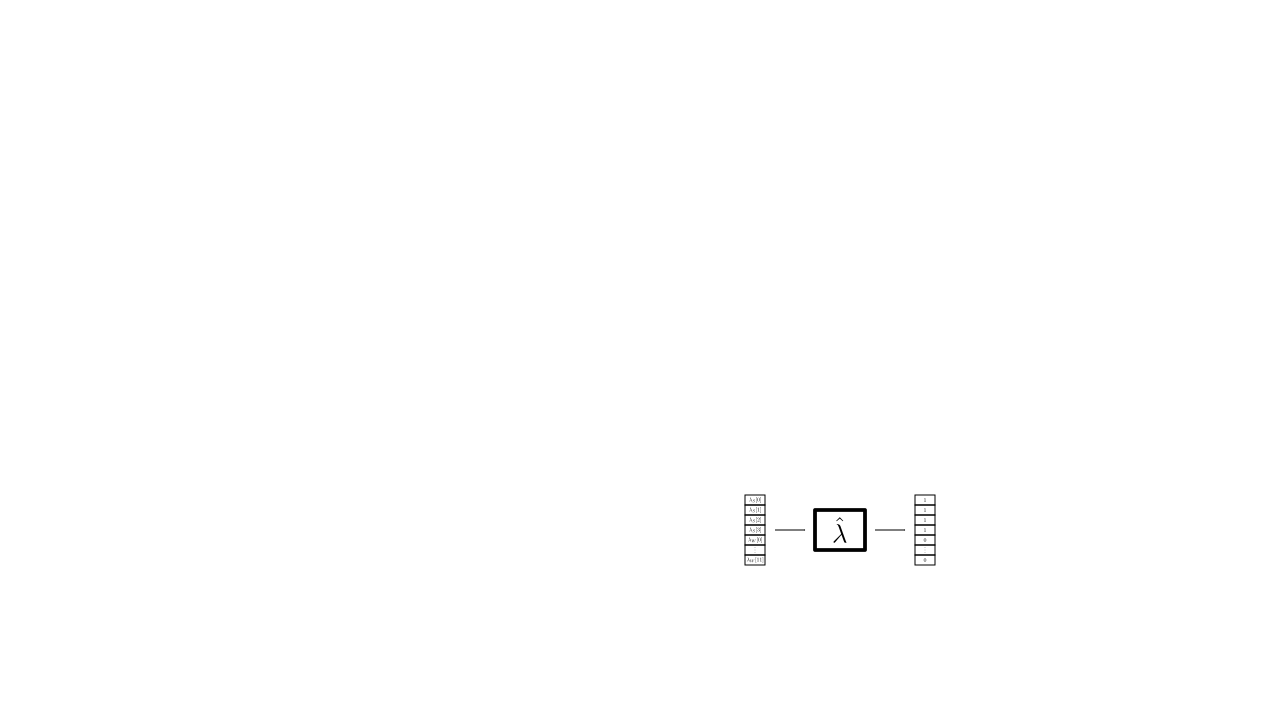
\includegraphics[width=0.7\linewidth]{images/05-Machine Learning/ml_maxder_imp.png}
  \caption{Esquema del estimador de cantidad de señales recibidas mediante el método de la máxima derivada visto como sistema para el caso de recepción de 4 señales. Se indican con $\lambda_S$ aquellos valores singulares correspondientes al subespacio de señal y con $\lambda_W$ aquellos que corresponden al subespacio de ruido.}
  \label{fig:ml_maxder_imp}
\end{figure}

Con esta simulación se compararon los vectores entregados por el algoritmo con los datos conocidos de los valores singulares clasificados para obtener una cuenta de los errores en la estimación y así obtener una medición de la precisión del algoritmo, la cual fue del 86,87\%.
%El error más probable que puede ocurrir en este algoritmo es que se detecten menos señales que las que existen en realidad. Siendo que la cantidad mínima de señales recibidas que entrega este algoritmo es 1 (ya que con alta probabilidad existirá un máximo en la derivada de la distribución), el error en esta técnica aumentará a medida que aumente la cantidad de señales recibidas. Una forma intuitiva de ver esto es pensar el caso en el que solo se recibe una única señal, en este caso el número mínimo que entregará el algoritmo será uno y esa señal será detectada el 100\% de las veces. Cuando se reciban dos señales, en el caso pesimista en el que solo se detecte una sola de ellas la precisión será del 50\%, y así sucesivamente.

\section{Clasificador binario mediante aprendizaje automático}

El problema de determinar si un valor singular corresponde al subespacio de ruido o al subespacio de señal se enmarca dentro de lo que en el campo del \emph{aprendizaje automático} o \emph{machine learning} se conoce como ``problema de clasificación binaria''.

En este tipo de problemas se intenta predecir el valor de una variable ``$y$'', de la cual se sabe que puede tomar dos valores, 0 y 1, que en este caso específico corresponden a la característica de si cada valor singular es un valor singular de ruido o de señal respectivamente, es decir:
\begin{equation}
  y=\left\{\begin{matrix}
    0 & \textrm{si corresponde a }\mathcal{S}_W \\
    1 & \textrm{si corresponde a }\mathcal{S}_S
  \end{matrix}\right.
\end{equation}
Esta predicción debe realizarse a partir de una entrada $\bar{x}$, la cual para esta aplicación en particular va a estar conformada por los parámetros que caracterizan a cada valor singular que se desea clasificar, y una hipótesis $h_{\bar{\theta}}(\bar{x})$ la cual no es más que una función que al recibir una entrada $\bar{x}$ entrega a la salida una predicción de la probabilidad de que $y$ sea igual a 1 para dicha entrada y para una elección de coeficientes representados en los elementos de un vector $\bar{\theta}$. Luego, configurando el umbral correspondiente, puede considerarse como $y=1$ a valores de probabilidad por encima de 0,5 y viceversa, y de esta forma se tiene el sistema clasificador que se indica en la Figura \ref{fig:ml_classificator_system}.
\begin{figure}[ht!]
  \centering
  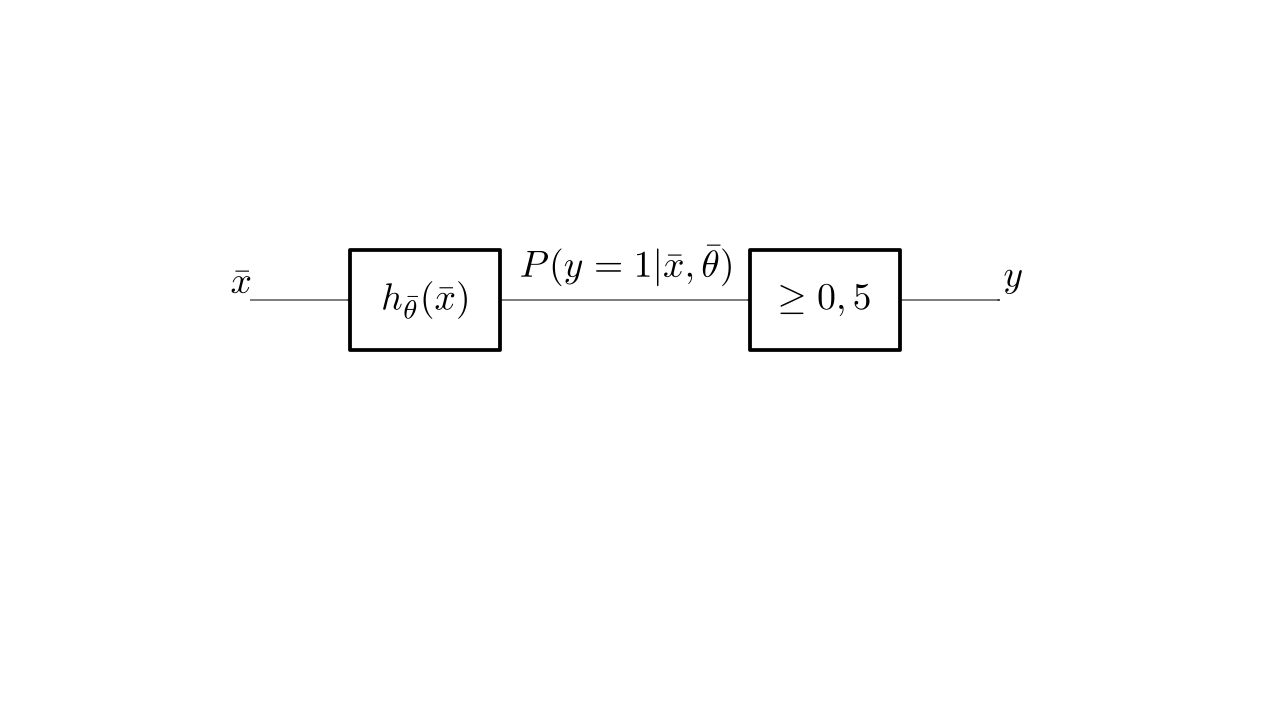
\includegraphics[width=0.7\linewidth]{images/05-Machine Learning/ml_classificator_system.png}
  \caption{Esquema de un clasificador utilizando aprendizaje automático visto como sistema.}
  \label{fig:ml_classificator_system}
\end{figure}

Existen varios tipos de algoritmos clasificadores, los cuales cada uno define su propia función de hipótesis $h_{\bar{\theta}}(\bar{x})$. A lo largo de este capítulo se analizarán dos de estos tipos; en primer lugar se explicará la técnica de \emph{Regresión Logística} para dar una introducción a los conceptos relacionados con el aprendizaje automático, y, finalmente, se analizará el algoritmo conocido como \emph{Máquina de Vectores de Soporte}, el cual es el algoritmo que finalmente se escogió para la implementación de este proyecto.

\subsection{Regresión Logística}
Debido a que la salida del clasificador es una variable que se encuentra contenida dentro del rango $[0,1]$ hay que definir una función para $h_{\bar{\theta}}(\bar{x})$ que cumpla con esta característica. El algoritmo de Regresión Logística define la siguiente función de hipótesis \cite{bib:machinelearning}:
\begin{gather}
  h_{\bar{\theta}}(\bar{x})=g(\bar{\theta}^T \bar{x}),\\
  g(z)=\frac{1}{1+e^{-z}},\end{gather}
donde $g(z)$ es conocida como la \emph{función sigmoide} o \emph{función lógística}, cuya forma se muestra en la Figura \ref{fig:ml_sigmoid}, y $\bar{\theta}$ es un vector de coeficientes a determinar.
\begin{figure}[ht!]
  \centering
  \includegraphics[width=0.9\linewidth]{images/05-Machine Learning/ml_sigmoid.png}
  \caption{Gráfica de la función sigmoide.}
  \label{fig:ml_sigmoid}
\end{figure}
Como se ve, esta función tiende a 1 para $z\rightarrow \infty$ y a 0 para $z\rightarrow -\infty$, y para $z=0$ vale 0,5.

El objetivo de todos los algoritmos de aprendizaje automático es el de ajustar los elementos del vector $\bar{\theta}$ de manera tal que la hipótesis genere una frontera de decisión que permita clasificar con la mayor precisión posible un conjunto de datos representados como vectores $\bar{x}$. Por ejemplo, si tenemos el conjunto de datos que se muestra en la Figura \ref{fig:ml_dataexample} se pueden definir los vectores:
\begin{equation*}
  \bar{x}=\begin{bmatrix}
    1     \\
    x_1   \\
    x_2   \\
    x_1^2 \\
    x_2^2
  \end{bmatrix},\quad
  \bar{\theta}=\begin{bmatrix}
    -1 \\
    0  \\
    0  \\
    1  \\
    1
  \end{bmatrix},
\end{equation*}
y de esta manera manera se tiene una función de hipótesis definida por:
\begin{equation*}
  h_{\bar{\theta}}(\bar{x})=g(\theta_0+\theta_1 x_1 + \theta_2 x_2 + \theta_3 x_1^2 + \theta_4 x_2^2) = g(-1+x_1^2+x_2^2)
\end{equation*}

Debido a lo que se ve en la Figura \ref{fig:ml_sigmoid}, la función sigmoide devuelve valores por encima de 0,5 para entradas mayores a 0. Por esto, para encontrar la frontera de decisión basta con ver los puntos del argumento de $g(\bar{\theta}^T \bar{x})$ tal que:
\begin{equation*}
  \bar{\theta}^T \bar{x} = -1+x_1^2+x_2^2 = 0,
\end{equation*}
y esos puntos son los que definen la frontera circular que se muestra en la Figura \ref{fig:ml_dataexample}.
\begin{figure}[ht!]
  \centering
  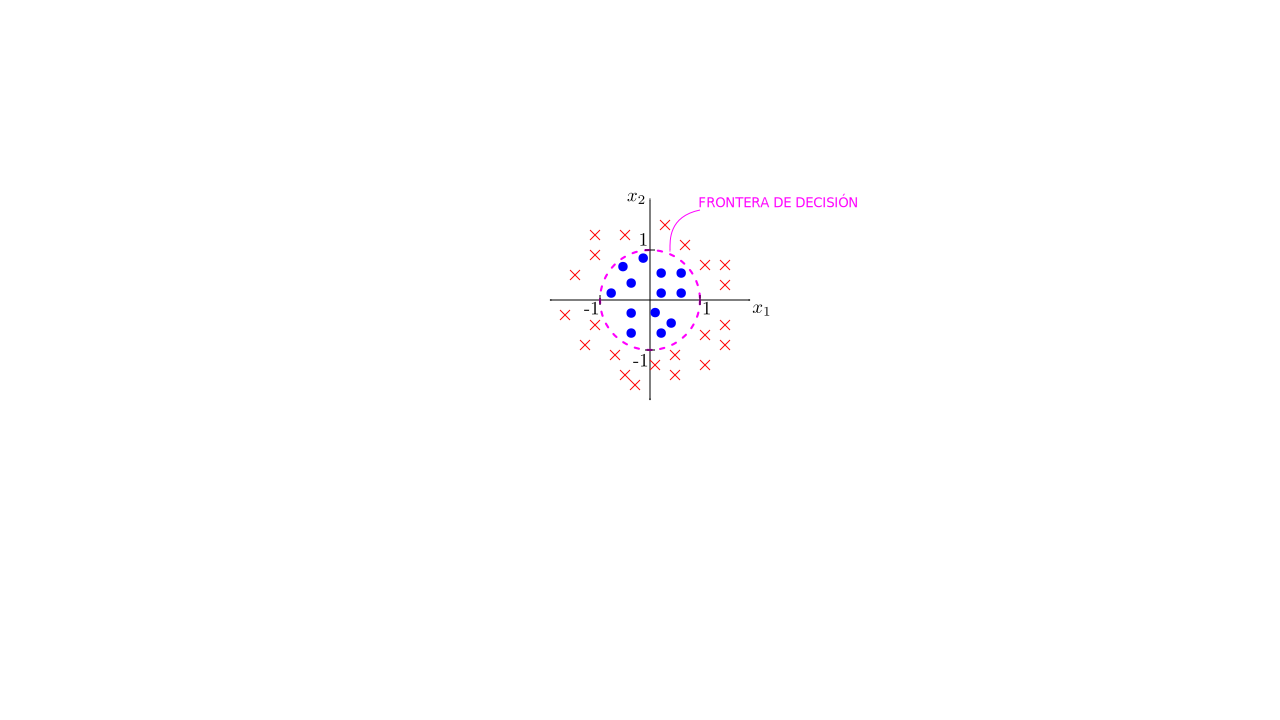
\includegraphics[width=0.8\linewidth]{images/05-Machine Learning/ml_dataexample.png}
  \caption{Ejemplo de frontera de decisión para un problema de clasificación binaria.}
  \label{fig:ml_dataexample}
\end{figure}

Vale la pena notar que en el ejemplo de la Figura \ref{fig:ml_dataexample} los datos a clasificar dependen de dos parámetros: $x_1$ y $x_2$. Sin embargo, el vector $\bar{x}$ no contiene únicamente estos dos parámetros sino que agrega nuevas \emph{características}, como lo son un término independiente $x_0=1$ y dos parámetros más que dependen de los originales: $x_1^2$ y $x_2^2$. Este método de agregar características polinomiales o términos rectangulares permite lograr fronteras de decisión más complejas que ajusten mejor a un determinado conjunto de datos, aunque pueden provocar un ``sobreajuste'' de los parámetros que degrade el comportamiento del clasificador al trabajar con datos que se encuentren fuera del conjunto de entrenamiento.

Como se dijo, el objetivo del aprendizaje automático consiste en ajustar los valores de $\bar{\theta}$ de manera tal de encontrar una frontera de decisión óptima. La manera de realizar este ajuste es entrenando al algoritmo a partir de un conjunto de datos llamado \emph{conjunto de entrenamiento}, de manera tal que, a medida de que el algoritmo itere, el error en la clasificación se reduzca. Para esto hay que definir una métrica de ese error, la cual es conocida como \emph{función de costo}. Para el algoritmo de regresión logística y teniendo un conjunto de datos de tamaño $M$ y una cantidad de características $N$, la función de costo está definida por \cite{bib:machinelearning}:
\begin{equation}
  J(\bar{\theta},\lambda)= -\frac{1}{M}\sum_{i=0}^{M-1} \left[y^{(i)} \log\left(h_{\bar{\theta}}(\bar{x}^{(i)})\right) + (1-y^{(i)}) \log\left(1-h_{\bar{\theta}}(\bar{x}^{(i)})\right) \right]+\frac{\lambda}{2M}\sum_{j=1}^{N-1}\theta_j^2,
  \label{eq:ml_costfunction}
\end{equation}
donde $y^{(i)}$ es la $i$-ésima variable que se desea predecir, $\bar{x}^{(i)}$ es el vector de entrada del clasificador correspondiente a la $i$-ésima variable a predecir, $\lambda$ es el \emph{parámetro de regularización} que permite suavizar la salida de la función de hipótesis para reducir el sobreajuste. Este parámetro también debe ser ajustado mediante entrenamiento. Finalmente, el problema a resolver consiste en encontrar los valores de $\bar{\theta}$ y $\lambda$ que minimicen la función de costo, es decir:
\begin{equation}
  \min_{\bar{\theta},\lambda} J(\bar{\theta},\lambda)
\end{equation}

Para minimizar la función de costo en regresión logística el procedimiento que se utiliza es el método de \emph{descenso de gradiente}, el cual es un algoritmo iterativo que permite acercarse con una cierta velocidad al mínimo de una función derivable. Utilizando esta técnica, la actualización de parámetros por cada iteración viene dada por:
\begin{equation}
  \begin{split}
    \theta_0 &:= \theta_0- \frac{\alpha}{M} \sum_{i=0}^{M-1}\left(h_{\bar{\theta}}(\bar{x}^{(i)})-y^{(i)}\right)x_0^{(i)}\\
    \theta_j &:= \theta_j- \frac{\alpha}{M} \left[\sum_{i=0}^{M-1} \left(h_{\bar{\theta}}(\bar{x}^{(i)})-y^{(i)}\right)x_j^{(i)}+\lambda\theta_j \right]\quad \textrm{para } j=1,...,N-1,
  \end{split}
\end{equation}
donde $\alpha$ es el \emph{coeficiente de aprendizaje} el cual se encarga de definir el tamaño de los ``pasos'' que se dan cuesta abajo en cada iteración del algoritmo. Si este $\alpha$ se elige muy grande es posible que el algoritmo nunca converja, y si se elige muy pequeño puede que tarde mucho tiempo en converger.
Es necesario ver que con este método no se actualiza el valor del parámetro $\lambda$. La manera de elegir un valor óptimo para este parámetro consiste en entrenar el algoritmo utilizando distintos valores de $\lambda$ y luego observar el rendimiento del clasificador utilizando datos que se encuentran fuera del conjunto de entrenamiento, eligiendo, finalmente, el valor de $\lambda$ que mejor ajuste este nuevo conjunto de datos, el cual es llamado \emph{conjunto de validación}.

\subsection{Máquina de Vectores de Soporte}\label{subc:ml_svm}
Uno de los algoritmos de clasificación más utilizados tanto en la industria como en la academia es el conocido como \emph{Máquina de Vectores de Soporte} (o \emph{SVM}, por sus siglas en inglés), el cual tiene la capacidad de poder entregar una mejor elección de una frontera de decisión a un menor costo comparado con el algoritmo de Regresión Logística. El algoritmo SVM toma la función de costos de la Ecuación \ref{eq:ml_costfunction}, y la simplifica de la siguiente manera:
\begin{equation}
  J(\bar{\theta},C)= C\sum_{i=0}^{M-1} \left[y^{(i)} \mathrm{cost}_1 (\bar{\theta}^T \bar{x}^{(i)}) + (1-y^{(i)}) \mathrm{cost}_0 (\bar{\theta}^T \bar{x}^{(i)}) \right]+\frac{1}{2}\sum_{j=1}^{N-1}\theta_j^2
  \label{eq:ml_costfunction_svm}
\end{equation}
donde $\mathrm{cost}_0(z)$ y $\mathrm{cost}_1(z)$ son las funciones que se indican en la Figura \ref{fig:ml_cost_svm} y $C = \frac{1}{\lambda}$.
\begin{figure}[ht!]
  \centering
  \begin{subfigure}[b]{0.49\textwidth}
    \centering
    \includegraphics[width=\linewidth]{images/05-Machine Learning/ml_cost1.png}
    \caption{$\mathrm{cost}_1(z)$}
  \end{subfigure}
  \hfill
  \begin{subfigure}[b]{0.49\textwidth}
    \centering
    \includegraphics[width=\linewidth]{images/05-Machine Learning/ml_cost0.png}
    \caption{$\mathrm{cost}_0(z)$}
  \end{subfigure}
  \caption{Cambios en la función de costo para SVM.}
  \label{fig:ml_cost_svm}
\end{figure}

Otra diferencia que tiene SVM con respecto a Regresión Logística es que la función de hipótesis en este caso no entrega una probabilidad sino directamente la predicción de $y$, es decir:
\begin{equation}
  h_{\bar{\theta}}(\bar{x})=\left\{\begin{matrix}
    0 & \textrm{si }\bar{\theta}^T \bar{x} < 0    \\
    1 & \textrm{si }\bar{\theta}^T \bar{x} \geq 0
  \end{matrix}\right.
  \label{eq:ml_hip_svm}
\end{equation}

Si se analizan la funciones $\mathrm{cost}_0(z)$ y $\mathrm{cost}_1(z)$ que se muestran en la Figura \ref{fig:ml_cost_svm} puede verse que la condición para que el primer término de la función de costos definida en la Ecuación \ref{eq:ml_costfunction_svm} se anule es:
\begin{equation}
  \begin{matrix}
    \bar{\theta}^T \bar{x}^{(i)}  \geq & 1  & \textrm{si } y^{(i)} = 1, \\
    \bar{\theta}^T \bar{x}^{(i)}  \leq & -1 & \textrm{si } y^{(i)} = 0.
  \end{matrix}
  \label{eq:ml_cond_svm}
\end{equation}

Cuando se resuelve el problema de optimización de minimizar la Ecuación \ref{eq:ml_costfunction_svm} resulta que la frontera de decisión que se obtiene utilizando SVM maximiza la distancia entre ella y los datos más cercanos a ella de cada una de las dos clases. Para dar un ejemplo de esto se muestra el conjunto de entrenamiento de la Figura \ref{fig:ml_db_svm}. Aquí vemos que en este caso de clasificación lineal pueden generarse infinitas rectas que logren una perfecta clasificación de este conjunto de datos, como las indicadas por las fronteras de color verde, sin embargo la frontera definida por SVM induce a pensar que va a lograr un mejor trabajo clasificando datos nuevos.
\begin{figure}[ht!]
  \centering
  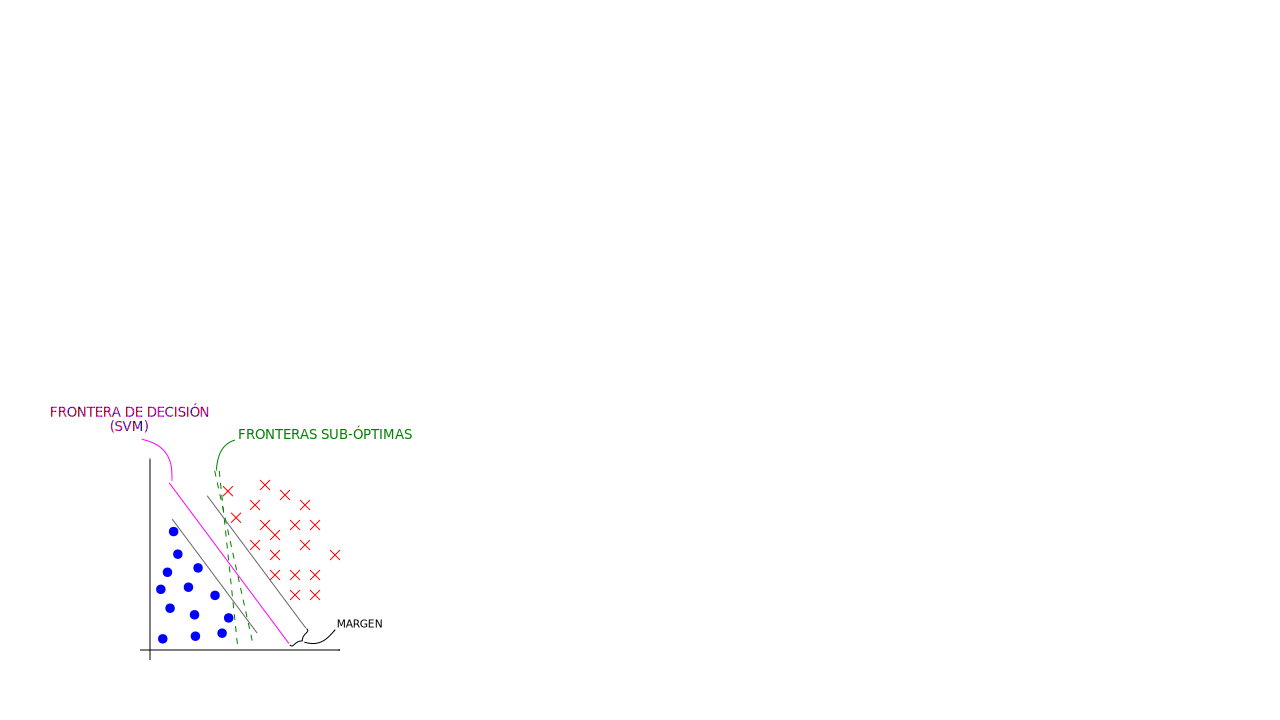
\includegraphics[width=0.8\linewidth]{images/05-Machine Learning/ml_db_svm.png}
  \caption{Frontera de decisión utilizando SVM.}
  \label{fig:ml_db_svm}
\end{figure}

De la Figura \ref{fig:ml_db_svm} se observa también que la frontera de decisión generada por SVM es la que maximiza el margen de separación entre datos rojos y azules. La razón por la cual ocurre esto tiene que ver con la condición definida en la Ecuación \ref{eq:ml_cond_svm} y la función de costos de la Ecuación \ref{eq:ml_costfunction_svm} ya que cumpliendo esas condiciones tenemos que la función de costo queda definida por:
\begin{equation}
  J(\bar{\theta})=\frac{1}{2} \sum_{j=1}^{N-1}\theta_j^2=\frac{1}{2} \left \|\bar{\theta} \right \|^2.
  \label{eq:ml_j_cost0}
\end{equation}
Además, las condiciones de la Ecuación \ref{eq:ml_cond_svm} pueden reescribirse como:
\begin{equation}
  \begin{matrix}
    p^{(i)} \cdot \left \| \bar{\theta} \right \| \geq & 1  & \textrm{si } y^{(i)} = 1, \\
    p^{(i)} \cdot \left \| \bar{\theta} \right \|\leq  & -1 & \textrm{si } y^{(i)} = 0,
  \end{matrix}
  \label{eq:ml_proyeccion_svm}
\end{equation}
donde $p^{(i)}$ es la proyección del vector $\bar{x}^{(i)}$ sobre el vector $\bar{\theta}$, o, lo que es lo mismo, la distancia del dato $\bar{x}^{(i)}$ a la frontera de decisión, debido a que la frontera de decisión es perpendicular a $\bar{\theta}$. Esto puede verse en el ejemplo de la Figura \ref{fig:ml_proyeccion_svm}.
\begin{figure}[ht!]
  \centering
  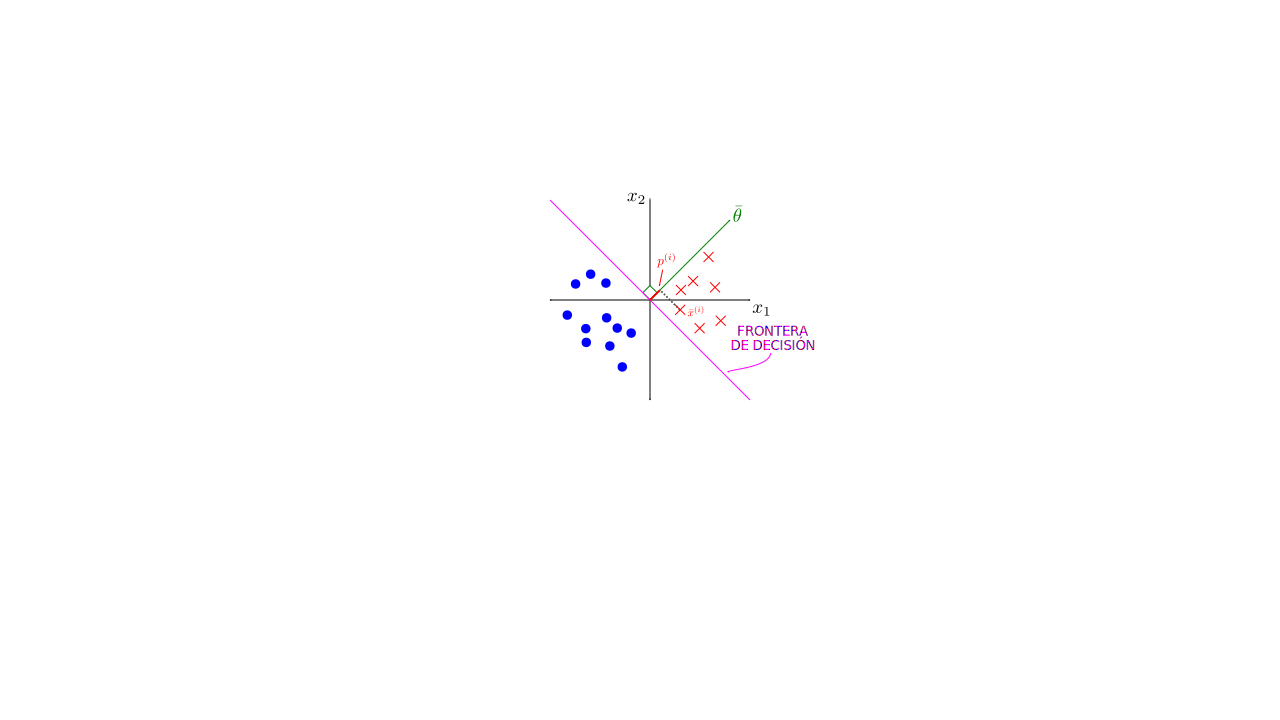
\includegraphics[width=0.7\linewidth]{images/05-Machine Learning/ml_proyeccion_svm.png}
  \caption{Proyección de un dato $\bar{x}^{(i)}$ sobre el vector $\bar{\theta}$ para un clasificador lineal con $\theta_0=0$.}
  \label{fig:ml_proyeccion_svm}
\end{figure}
Si algún dato $\bar{x}^{(i)}$ se encontrara sobre la frontera de decisión estaría ubicado numéricamente en el salto de la función de hipótesis definida en la Ecuación \ref{eq:ml_hip_svm}, lo que significa que para puntos definidos por vectores $\bar{x}^{(i)}$ que se encuentren dentro de la frontera de decisión, el producto escalar $\bar{\theta}^T \bar{x}$ vale 0, lo que indica que todos los puntos dentro de la frontera de decisión son ortogonales a $\bar{\theta}$.

A partir de aquí se observa que al minimizar la Ecuación \ref{eq:ml_j_cost0} se minimiza la norma de $\bar{\theta}$, por ende para cumplir las condiciones de la Ecuación \ref{eq:ml_proyeccion_svm} al minimizarse $\left\| \bar{\theta} \right \|$ debe maximizarse $p^{(i)}$, lo que significa maximizar la distancia entre los datos del conjunto de entrenamiento y la frontera de decisión.

Finalmente, SVM implementa una nueva manera de definir las características del vector $\bar{x}$ distinta a la manera polinomial que se vio en Regresión Logística. Teniendo un conjunto de $M$ datos de entrenamiento se define el vector de características de un dato $\bar{f}^{(i)}\in \mathbb{R}^{M\times 1}$ para $i=0,1,...,M-1$ como:
\begin{equation}
  \bar{f}^{(i)}=\begin{bmatrix}
    f_0^{(i)} \\
    f_1^{(i)} \\
    \vdots    \\
    f_{M-1}^{(i)}
  \end{bmatrix}_{(M\times 1)} ,
\end{equation}
donde $f_j^{(i)}=k(\bar{x}^{(i)},\bar{x}^{(j)})$ es una función que mide la ``semejanza'' entre el dato $\bar{x}^{(i)}$ y el dato $\bar{x}^{(j)}$, la cual es llamada \emph{función kernel}. Ahora la función de hipótesis queda definida por:
\begin{equation}
  h_{\bar{\theta}}(\bar{f})=\left\{\begin{matrix}
    0 & \textrm{si }\bar{\theta}^T \bar{f} < 0    \\
    1 & \textrm{si }\bar{\theta}^T \bar{f} \geq 0
  \end{matrix}\right.
  \label{eq:ml_hipkernel_svm}
\end{equation}

Debe notarse que ahora la dimensión del vector $\bar{\theta}$ es igual a la cantidad de datos del conjunto de entrenamiento, entonces la función de costo de la Ecuación \ref{eq:ml_costfunction} puede reescribirse como:
\begin{equation}
  J(\bar{\theta},C)= C\sum_{i=0}^{M-1} \left[y^{(i)} \mathrm{cost}_1 (\bar{\theta}^T \bar{f}^{(i)}) + (1-y^{(i)}) \mathrm{cost}_0 (\bar{\theta}^T \bar{f}^{(i)}) \right]+\frac{1}{2}\sum_{j=1}^{M-1}\theta_j^2
  \label{eq:ml_costfunctionkernel_svm}
\end{equation}

Existen múltiples maneras de definir la función kernel, donde cada una se ajusta mejor a ciertos tipos de distribuciones de datos. Algunos de los tipos de kernels más comunes son \cite{bib:sklearn_svm}:
\begin{itemize}
  \item \textbf{Kernel Lineal :=} $k_{\textrm{lineal}}(\bar{x}^{(i)},\bar{x}^{(j)})=\left \langle \bar{x}^{(i)},\bar{x}^{(j)} \right \rangle$
  \item \textbf{Kernel Gaussiano :=} $k_{\textrm{gaussiano}}(\bar{x}^{(i)},\bar{x}^{(j)})=-\gamma \left \| \bar{x}^{(i)}-\bar{x}^{(j)} \right \|^2$, con $\gamma>0$
  \item \textbf{Kernel Polinomial :=} $k_{\textrm{polinomial}}(\bar{x}^{(i)},\bar{x}^{(j)})=\left( \gamma \left \langle \bar{x}^{(i)},\bar{x}^{(j)} \right \rangle +r \right)^d$, siendo $d$ el grado del polinomio y $r$ un término independiente.
  \item \textbf{Kernel Sigmoide :=} $k_{\textrm{sigmoide}}(\bar{x}^{(i)},\bar{x}^{(j)})=\tanh{\left(\gamma \left \langle \bar{x}^{(i)},\bar{x}^{(j)} \right \rangle +r\right)}$

\end{itemize}

En la actualidad existen múltiples librerías con implementaciones optimizadas de algoritmos de SVM para distintos tipos de kernels escritos en una gran variedad de lenguajes, como lo son la librería \texttt{scikit-learn} \cite{bib:sklearn_svm} en \texttt{Python} o \texttt{LIBSVM} \cite{bib:LIBSVM} en \texttt{C++}, lo cual hace que la implementación de estos algoritmos pueda realizarse de forma muy rápida.

\subsection{Resultados obtenidos}
%Feature scaling
% Método de testeo: training set - cross validations set - test set
% 6 week
%Training set: 60%
%Cross validation set: 20%
%Test set: 20% 

En esta sección se muestran los resultados obtenidos luego de aplicar las técnicas de estimación de cantidad de señales recibidas mediante aprendizaje automático. En este caso solo se realizó el análisis del algoritmo SVM debido a su simplicidad de implementación con respecto a Regresión Logística.

Para poder operar con estas técnicas primero deben elegirse las características que definen a cada valor singular a clasificar. La primer característica a definir es la magnitud del mismo, ya que cuanto más grande sea, mayor va a ser la probabilidad de que sea un valor singular correspondiente al subespacio de señal. Sin embargo esta característica no es suficiente, ya que, según cómo sean las propiedades de las señales recibidas, el piso de ruido puede variar de manera tal de que lo que antes era una magnitud que correspondía a un valor singular de señal en otro caso puede corresponder a un valor singular de ruido. Por ende hay que definir una nueva característica que tenga en cuenta la relación de magnitudes entre los valores singulares de ruido y de señal en cada descomposición de valores singulares. Según lo que se definió en la Ecuación \ref{eq:doaest_aval}, en la descomposición en autovalores de la matriz $\mathbf{R_{XX}}$ definida en la Ecuación \ref{eq:doaest_rxx_teor} los autovalores máximos y mínimos vienen dados por:
\begin{align}
  \lambda_{\textrm{máx}} & = M \cdot |s_{\textrm{máx}}|^2+\sigma_w^2, \\
  \lambda_{\textrm{mín}} & = \sigma_w^2.
\end{align}
Por ende, a partir de estos valores puede definirse una noción de SNR haciendo:
\begin{equation}
  \hat{\mathrm{SNR}} = \frac{\lambda_{\textrm{máx}}-\lambda_{\textrm{mín}}}{M\cdot \lambda_{\textrm{mín}}}=\frac{|s_{\textrm{máx}}|^2}{\sigma_w^2}
  \label{eq:ml_svm_snrhat}
\end{equation}
Hay que tener en cuenta que esta definición no indica una SNR per se, ya que $\lambda_{\textrm{máx}}$ solo contiene información de la señal que arriba con mayor potencia e ignora a las otras, pero esta diferencia de magnitudes permite aportar información de utilidad que permita realizar la clasificación de los valores singulares. Además, siendo que se trabaja con una cantidad de muestras finitas, los autovalores de la matriz de covarianza muestral definida en la Ecuación \ref{eq:doaest_rxx_est} no serán iguales a lo que se mostró en la Ecuación \ref{eq:doaest_aval} y ocurrirá que los autovalores de ruido contendrán información de las señales y viceversa. Sin embargo, la práctica demuestra que es una buena métrica que puede usarse como característica. Como en la Sección \ref{subc:doaest_datamodel} se decidió que la descomposición del subespacio se realiza aplicando directamente la SVD sobre la matriz $\mathbf{X}$ definida en la Ecuación \ref{eq:doaest_x}, no se puede definir exactamente la misma SNR de la Ecuación \ref{eq:ml_svm_snrhat}, ya que los valores singulares de $\mathbf{X}$ no son iguales a los autovalores de $\mathbf{\hat{R}_{XX}}$, sin embargo, estos están relacionados de la siguiente manera \cite{bib:strang}:
\begin{equation}
  \sigma_{\mathbf{X}} = \sqrt{|\lambda_{\mathbf{\hat{R}_{XX}}}|},
\end{equation}
siendo $\sigma_{\mathbf{X}}$ los valores singulares de $\mathbf{X}$ y $\lambda_{\mathbf{\hat{R}_{XX}}}$ los autovalores de $\mathbf{\hat{R}_{XX}}$. Entonces, utilizando los valores singulares de la SVD de $\mathbf{X}$ se puede redefinir la SNR de la Ecuación \ref{eq:ml_svm_snrhat} de la siguiente forma:
\begin{equation}
  \hat{\mathrm{SNR}} = \frac{\sigma^2_{\textrm{máx}}}{\sigma^2_{\textrm{mín}}},
  \label{eq:ml_svm_snrhatsvd}
\end{equation}
donde $\sigma_{\textrm{máx}}$ y $\sigma_{\textrm{mín}}$ son los valores singulares máximos y mínimos, respectivamente, de cada SVD realizada sobre cada matriz de muestras $\mathbf{X}$.

A partir de estas dos características ahora puede definirse un vector de entrada para el clasificador de la siguiente manera:
\begin{equation}
  \bar{x}^{(i)}=\begin{bmatrix}
    \lambda^{(i)} \\
    \hat{\mathrm{SNR}}^{(i)}
  \end{bmatrix}
  \label{eq:ml_svm_x}
\end{equation}
con $i=0,1,...,M-1$, y siendo $M$ el tamaño del conjunto de datos.

Utilizando la misma base de valores singulares que se generó en la Sección \ref{subc:ml_maxder_resul} y en función de la definición de la Ecuación \ref{eq:ml_svm_x}, puede realizarse la gráfica de la Figura \ref{fig:ml_avals_plot}, en donde se representan 2000 valores singulares correspondientes al subespacio de ruido y 2000 valores singulares correspondientes al subespacio de señal elegidos al azar en función de las características definidas. Como puede verse en esta gráfica, existen dos zonas bien separadas que pueden utilizarse para definir una frontera de decisión. Los valores singulares de ruido se ubican sobre el margen izquierdo de la gráfica, la cual corresponde a valores singulares de magnitud pequeña, y los autovalores de señal se extienden por toda la gráfica hacia la derecha, tomando diferentes valores según la potencia de la señal que representan.
\begin{figure}[ht!]
  \centering
  \includegraphics[width=0.9\linewidth]{images/05-Machine Learning/ml_avals_plot.png}
  \caption{Gráfica de valores singulares de distintas realizaciones de $\mathbf{X}$ en función de las características definidas para el problema de clasificación mediante aprendizaje automático.}
  \label{fig:ml_avals_plot}
\end{figure}

Antes de comenzar con el entrenamiento del algoritmo es necesario preparar los datos para que las iteraciones minimicen la función de costo de la manera más rápida. Para lograr esto se utilizará la técnica de \emph{escalamiento de características} \cite{bib:machinelearning}, que consiste en normalizar los rangos de variación de los valores de las características del conjunto de entrenamiento para que ambos varíen en una misma escala. Para eso se procede definiendo las siguientes magnitudes:
\begin{equation}
  \begin{gathered}
    \mu_{\lambda}=\frac{1}{M_{\textrm{tr}}} \sum_{i=0}^{M_{\textrm{tr}-1}} \lambda^{(i)},\quad \mu_{\hat{\mathrm{SNR}}}=\frac{1}{M_{\textrm{tr}}} \sum_{i=0}^{M_{\textrm{tr}-1}} \hat{\mathrm{SNR}}^{(i)}\\
    \sigma_{\lambda}=\max(\bar{\lambda})-\min(\bar{\lambda}),\quad \sigma_{\hat{\mathrm{SNR}}}=\max(\bar{\mathrm{SNR}})-\min(\bar{\mathrm{SNR}}),
  \end{gathered}
\end{equation}
donde $\mu_{\lambda}$ es el valor medio de las magnitudes de todos los valores singulares en el conjunto de entrenamiento, $\mu_{\hat{\mathrm{SNR}}}$ es el valor medio de la $\hat{\mathrm{SNR}}$ de todos los valores singulares del conjunto de entrenamiento como se definió en la Ecuación \ref{eq:ml_svm_snrhat}, $\sigma_{\lambda}$ es la diferencia entre la magnitud del valor singular máximo y mínimo del conjunto de entrenamiento, $\sigma_{\hat{\mathrm{SNR}}}$ es la diferencia entre el valor de $\hat{\mathrm{SNR}}$ máximo y mínimo de todo el conjunto de entrenamiento, y $M_{\textrm{tr}}$ es el tamaño del conjunto de entrenamiento. Luego de definir estas variables se afecta a cada vector $\bar{x}^{(i)}$ del conjunto total de datos de la siguiente manera:
\begin{gather}
  \bar{x}_{fs}^{(i)}=\mathbf{\Sigma} \cdot \left( \bar{x}^{(i)} - \bar{\mu}  \right)=\begin{bmatrix}
    \frac{\lambda^{(i)}-\mu_{\lambda}}{\sigma_{\lambda}} \\
    \frac{\hat{\mathrm{SNR}}-\mu_{\hat{\mathrm{SNR}}}}{\sigma_{\hat{\mathrm{SNR}}}}
  \end{bmatrix}\\
  \mathbf{\Sigma}=\begin{bmatrix}
    \frac{1}{\sigma_{\lambda}} & 0                                     \\
    0                          & \frac{1}{\sigma_{\hat{\mathrm{SNR}}}}
  \end{bmatrix},\quad \bar{\mu}=\begin{bmatrix}
    \mu_{\lambda} \\
    \mu_{\hat{\mathrm{SNR}}}
  \end{bmatrix}\nonumber
\end{gather}


Luego de acondicionar los datos se definieron los conjuntos de entrenamiento, validación y prueba de la siguiente manera:
\begin{itemize}
  \item \textbf{Conjunto de entrenamiento:} 60\% del conjunto total de datos. Es el utilizado para obtener los elementos del vector de parámetros $\bar{\theta}$ mediante entrenamiento del algoritmo.
  \item \textbf{Conjunto de validación:} 20\% del conjunto total de datos. Se utiliza para ajustar los coeficientes y términos independientes propios de cada kernel.
  \item \textbf{Conjunto de prueba}: 20\% del conjunto total de datos. Se utiliza para medir la precisión del algoritmo.
\end{itemize}

Utilizando los conjuntos de entrenamiento y validación se entrenó el algoritmo SVM utilizando distintos kernels, obteniendo los resultados que se muestran a continuación.

\subsubsection{Kernel Sigmoide}

Luego de entrenar al algoritmo utilizando este kernel se llegó a la elección de parámetros $C=30$, $\gamma=0,3$ y $r=0,01$. A partir de estos parámetros y la obtención del vector $\bar{\theta}$ mediante entrenamiento del algoritmo se obtuvo la frontera de decisión que se muestra en la Figura \ref{fig:ml_svm_sigmoid}.

\begin{figure}[ht!]
  \centering
  \includegraphics[width=0.9\linewidth]{images/05-Machine Learning/ml_svm_sigmoid.png}
  \caption{Frontera de decisión definida por el algoritmo SVM utilizando un kernel sigmoide}
  \label{fig:ml_svm_sigmoid}
\end{figure}

Comparando las características conocidas del conjunto de datos se evaluó la precisión del clasificador utilizándolo en distintos conjuntos de prueba obteniendo los siguientes resultados:
\begin{itemize}
  \item \textbf{Conjunto de prueba:} 96,70\% de precisión.
  \item \textbf{Conjunto de validación:} 96,60\% de precisión.
  \item \textbf{Conjunto de entrenamiento:} 96,71\% de precisión.
  \item \textbf{Todos los datos:} 96,69\% de precisión.
\end{itemize}

\subsubsection{Kernel Polinomial}
Realizando numerosas iteraciones se optimizó el algoritmo SVM utilizando un kernel polinomial con los parámetros $C=0,03$, $d=4$, $\gamma=50$, $r=1$. En la Figura \ref{fig:ml_svm_poly} se muestra la frontera de decisión obtenida con este clasificador. Como puede observarse, esta frontera no pareciera mostrar un resultado adecuado en la zona inferior izquierda e inferior derecha de la gráfica, esto se debe a la falta de valores singulares en esa zona que ayuden a aportar información al algoritmo.

\begin{figure}[ht!]
  \centering
  \includegraphics[width=0.9\linewidth]{images/05-Machine Learning/ml_svm_poly.png}
  \caption{Frontera de decisión definida por el algoritmo SVM utilizando un kernel polinomial.}
  \label{fig:ml_svm_poly}
\end{figure}

\begin{itemize}
  \item \textbf{Conjunto de prueba:} 96,85\% de precisión.
  \item \textbf{Conjunto de validación:} 97,15\% de precisión.
  \item \textbf{Conjunto de entrenamiento:} 96,92\% de precisión.
  \item \textbf{Todos los datos:} 96,95\% de precisión.
\end{itemize}

\subsubsection{Kernel Gaussiano}
Luego de entrenar al algoritmo se fijaron los parámetros $C=50$ y $\gamma=30$. En la Figura \ref{fig:ml_svm_rbf} se indica la frontera de decisión definida por este kernel junto con el conjunto de datos clasificado.

\begin{figure}[ht!]
  \centering
  \includegraphics[width=0.9\linewidth]{images/05-Machine Learning/ml_svm_rbf.png}
  \caption{Frontera de decisión definida por el algoritmo SVM utilizando un kernel gaussiano.}
  \label{fig:ml_svm_rbf}
\end{figure}

Contando los errores producidos al clasificar los distintos conjuntos de datos se obtuvieron las siguientes medidas de precisión:
\begin{itemize}
  \item \textbf{Conjunto de prueba:} 96,92\% de precisión.
  \item \textbf{Conjunto de validación:} 97,25\% de precisión.
  \item \textbf{Conjunto de entrenamiento:} 97,12\% de precisión.
  \item \textbf{Todos los datos:} 97,11\% de precisión.
\end{itemize}

Con las simulaciones realizadas puede concluirse que este es el kernel que alcanzó la mayor precisión. Sin embargo, el entrenamiento del algoritmo con datos simulados no es suficiente para llevar este clasificador a una implementación real. En ese caso lo correcto será volver a entrenar al mismo utilizando mediciones reales de las señales satelitales que se desea recibir.